% Chapter Template

\chapter{Literature Review} % Main chapter title

\label{Chapter2} % Change X to a consecutive number; for referencing this chapter elsewhere, use \ref{ChapterX}

\lhead{Chapter 2. \emph{Literature Review}} % Change X to a consecutive number; this is for the header on each page - perhaps a shortened title

%----------------------------------------------------------------------------------------
%	SECTION 1
%----------------------------------------------------------------------------------------

\section{Introduction}
%\begin{figure}[h]
%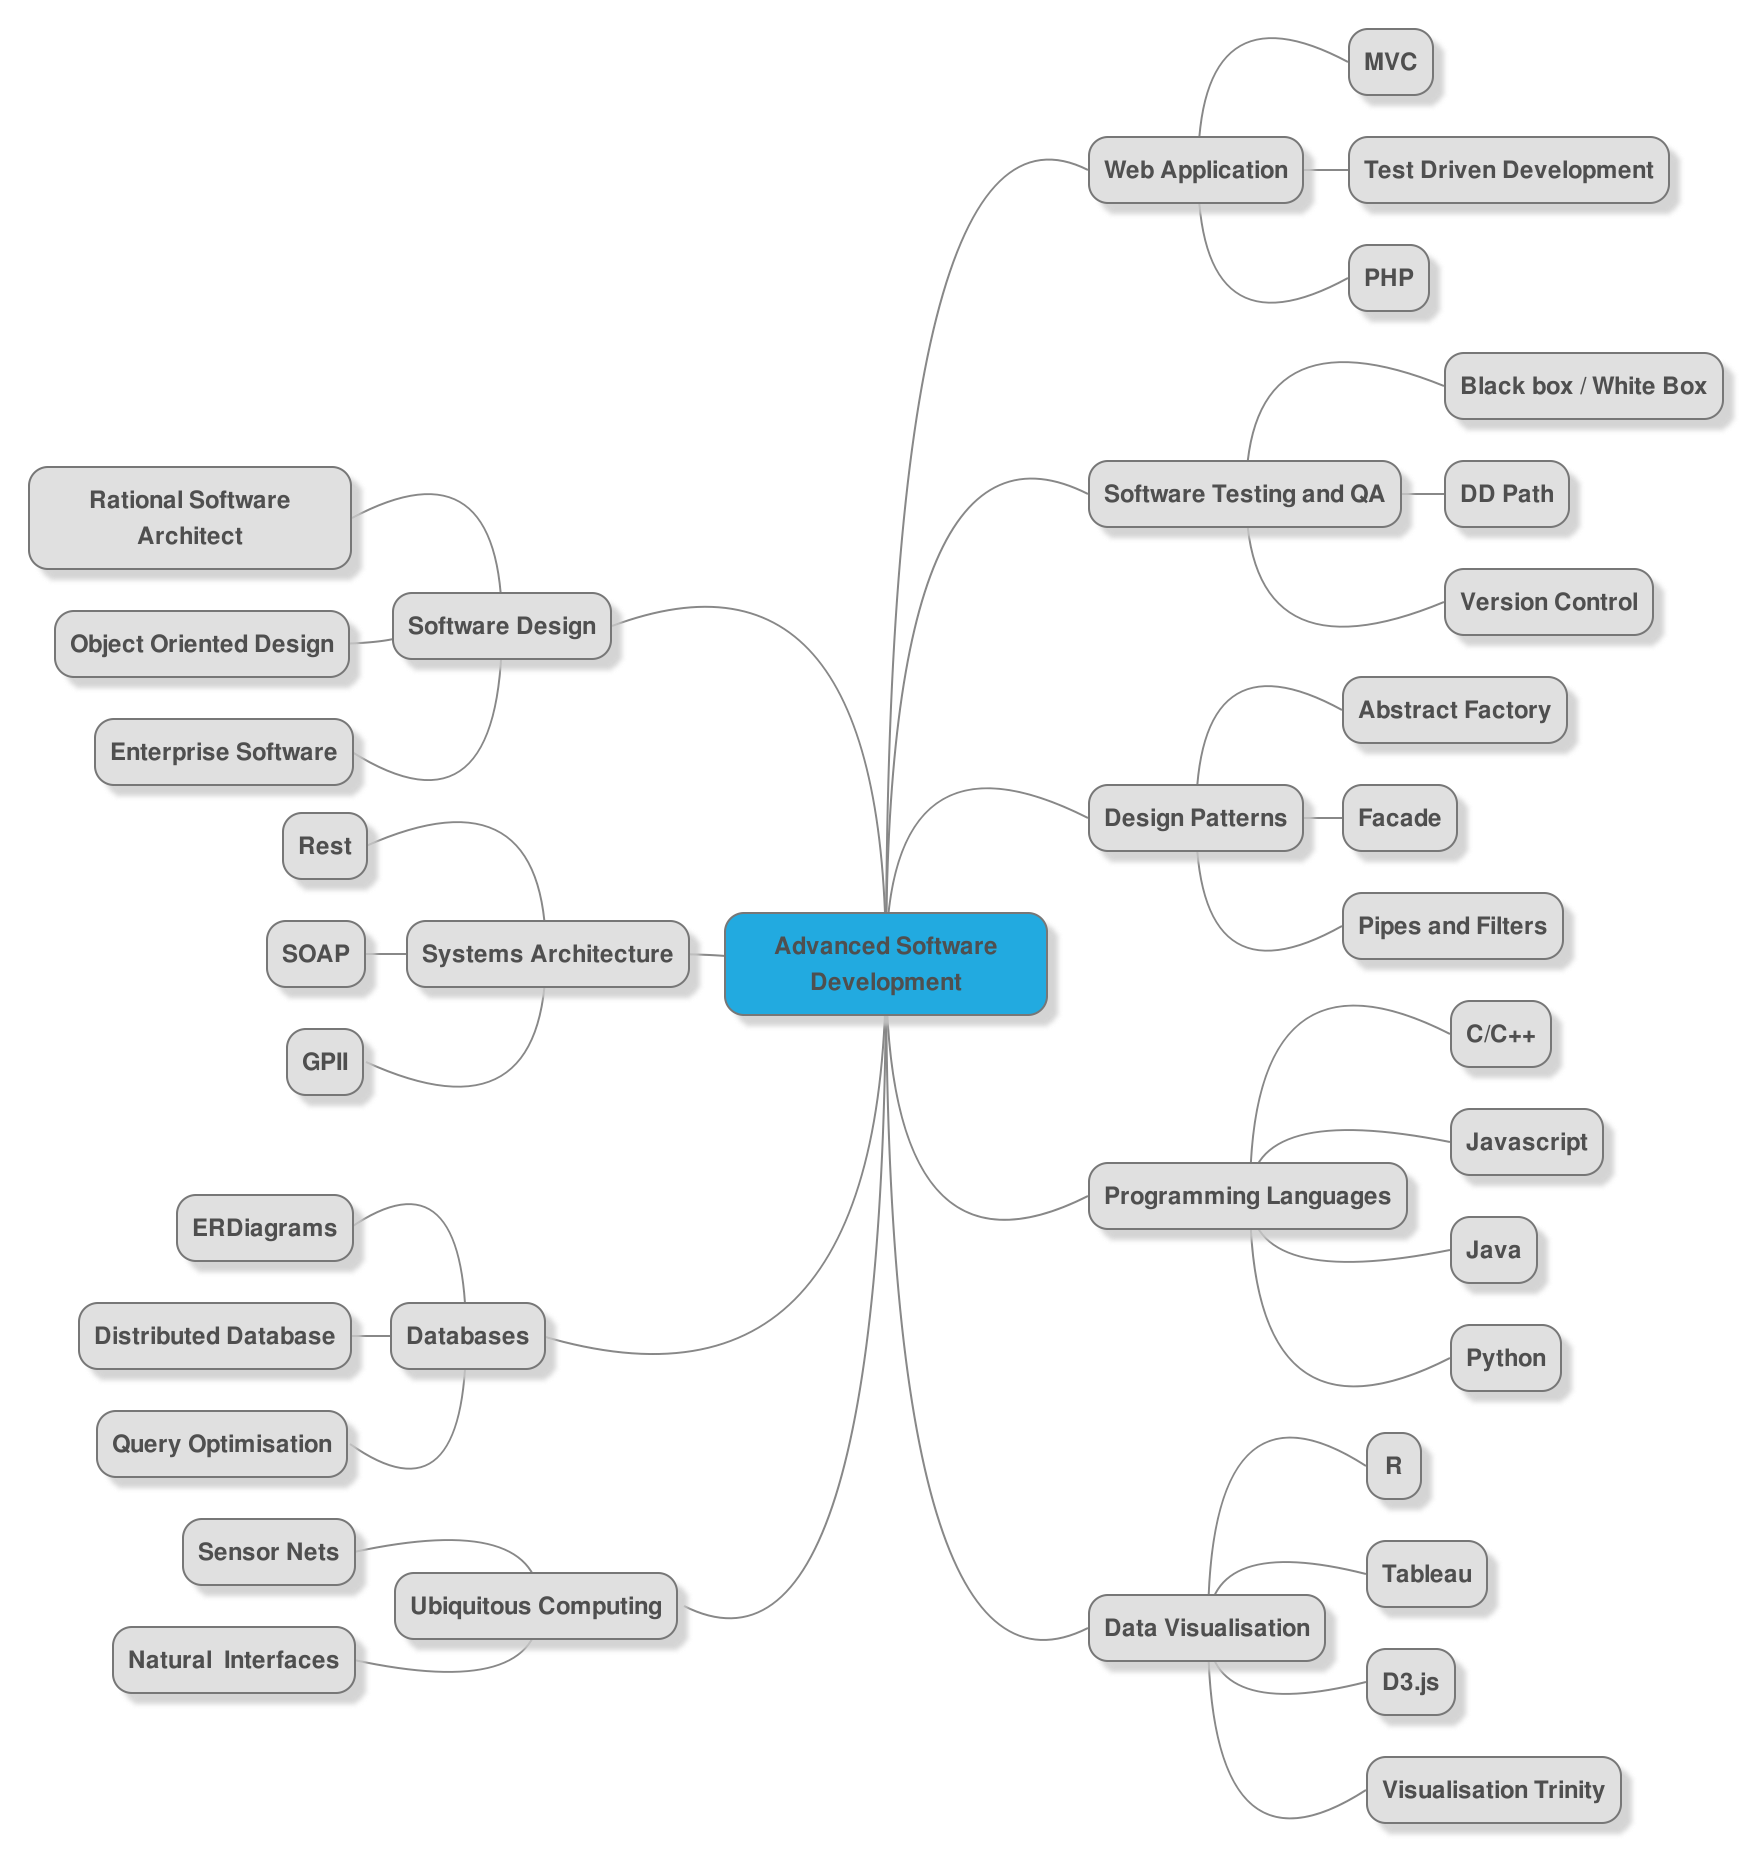
\includegraphics[scale=.2]{mindmap}
%\caption{A mind map of my discipline}
%\centering
%\end{figure}
%-----------------------------------
%	MACHINE LEARNING
%-----------------------------------
\section{Machine Learning}

Swedish researchers perform interviews with developers in several different companies to increase the understanding in the area of market driven requirements engineering.\cite{Interview1}
Researchers conduct semi-structured interviews in order to understand the management challenges associated with outsourcing software development.\cite{Interview2}

\subsection{}

\subsection{}

\subsection{}

\subsection{}

\subsection{}

%-----------------------------------
%	ARGUMENTATION THEORY
%-----------------------------------

\section{Argumentation Theory}

Contributors to the Linux kernel answer an online questionnaire about the motives in contributing to open source and identify 7 factors that contribute to the motivation.\cite{Questionnaire1}
American Researchers use surveys to determine the effect of multi site software development. The results show that multi site software development requires more staff and takes longer than typical software development.\cite{Questionnaire2}

\subsection{Argumentation Theory in AI}

\subsection{Non-Monotonic Reasoning}

\subsection{Defeasible Reasoning}


%----------------------------------------------------------------------------------------
%	CONCLUSIONS
%----------------------------------------------------------------------------------------

\section{Conclusions}

Sed ullamcorper quam eu nisl interdum at interdum enim egestas. Aliquam placerat justo sed lectus lobortis ut porta nisl porttitor. Vestibulum mi dolor, lacinia molestie gravida at, tempus vitae ligula. Donec eget quam sapien, in viverra eros. Donec pellentesque justo a massa fringilla non vestibulum metus vestibulum. Vestibulum in orci quis felis tempor lacinia. Vivamus ornare ultrices facilisis. Ut hendrerit volutpat vulputate. Morbi condimentum venenatis augue, id porta ipsum vulputate in. Curabitur luctus tempus justo. Vestibulum risus lectus, adipiscing nec condimentum quis, condimentum nec nisl. Aliquam dictum sagittis velit sed iaculis. Morbi tristique augue sit amet nulla pulvinar id facilisis ligula mollis. Nam elit libero, tincidunt ut aliquam at, molestie in quam. Aenean rhoncus vehicula hendrerit.
